%!TEX root = Report.tex
\chapter{MATLAB Code}\label{c:datasheets}


 %\lstinputlisting{hightemp2.m}

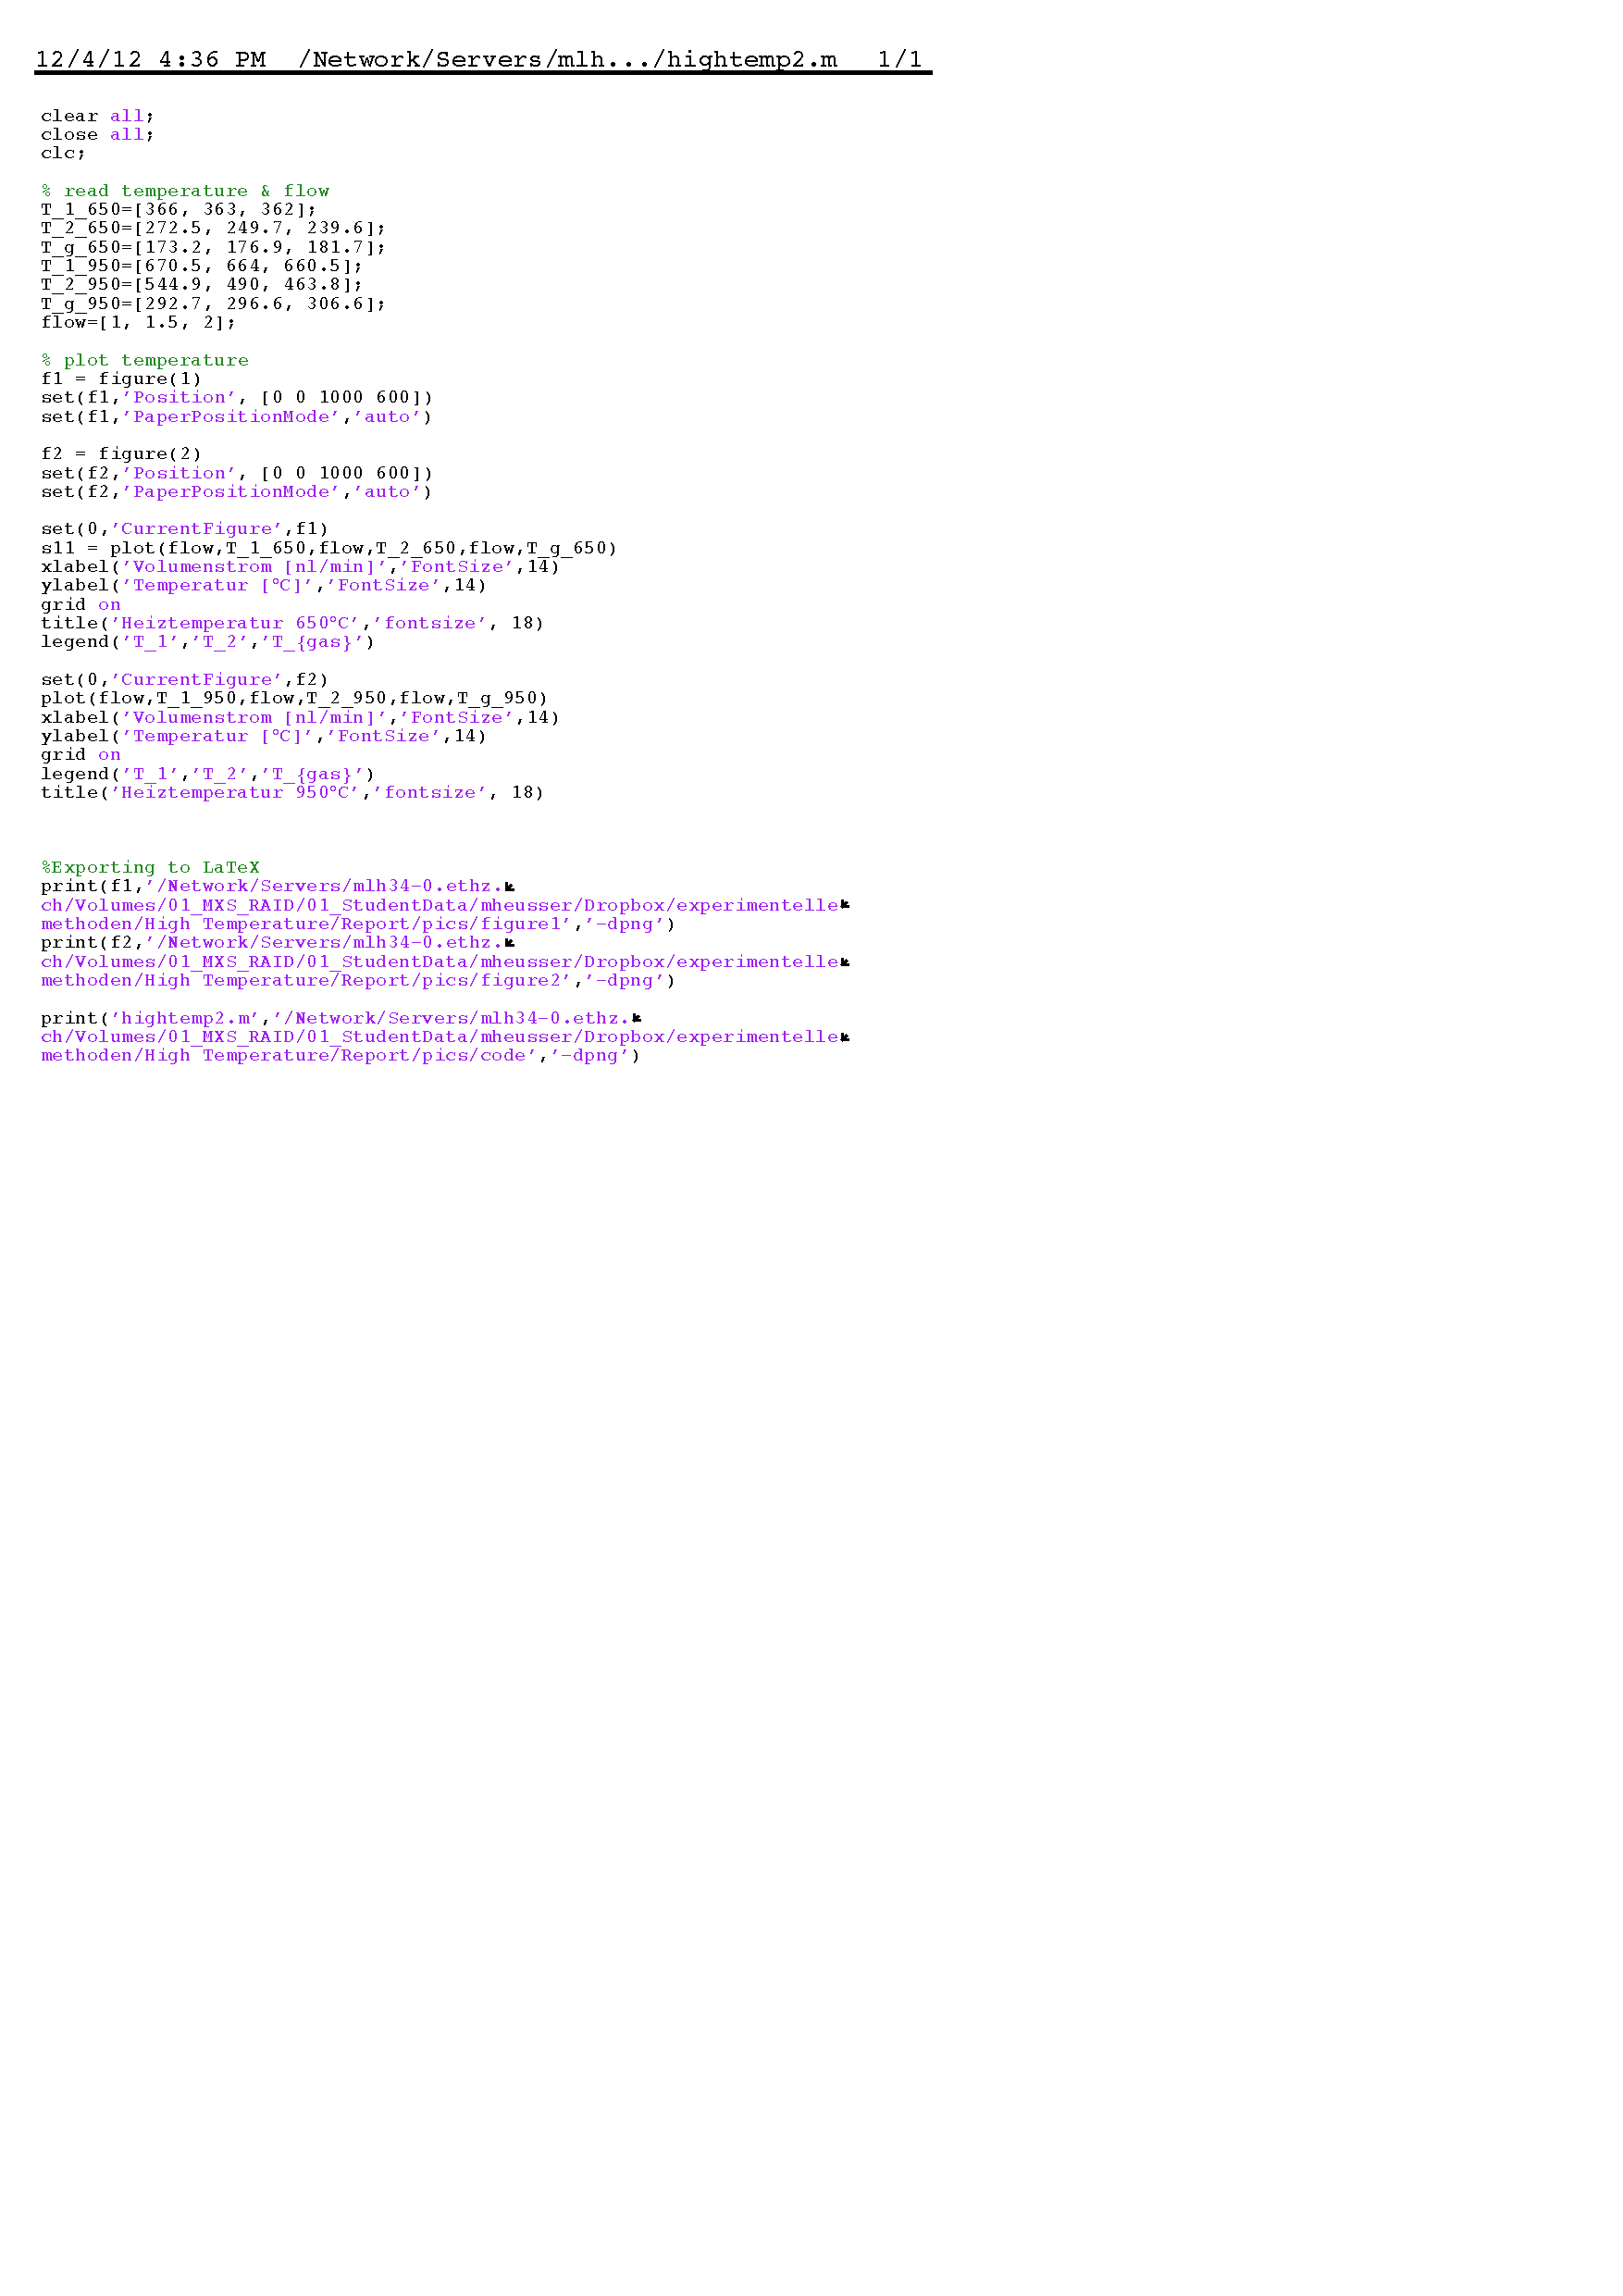
\includepdf[pages=-,frame=true, scale=0.9]{pics/code.pdf}

%\includepdf[pages={1,3,4-5},angle=0,nup=2x2,frame=true, scale=0.9]{datasheets/PicDatasheet.pdf}
%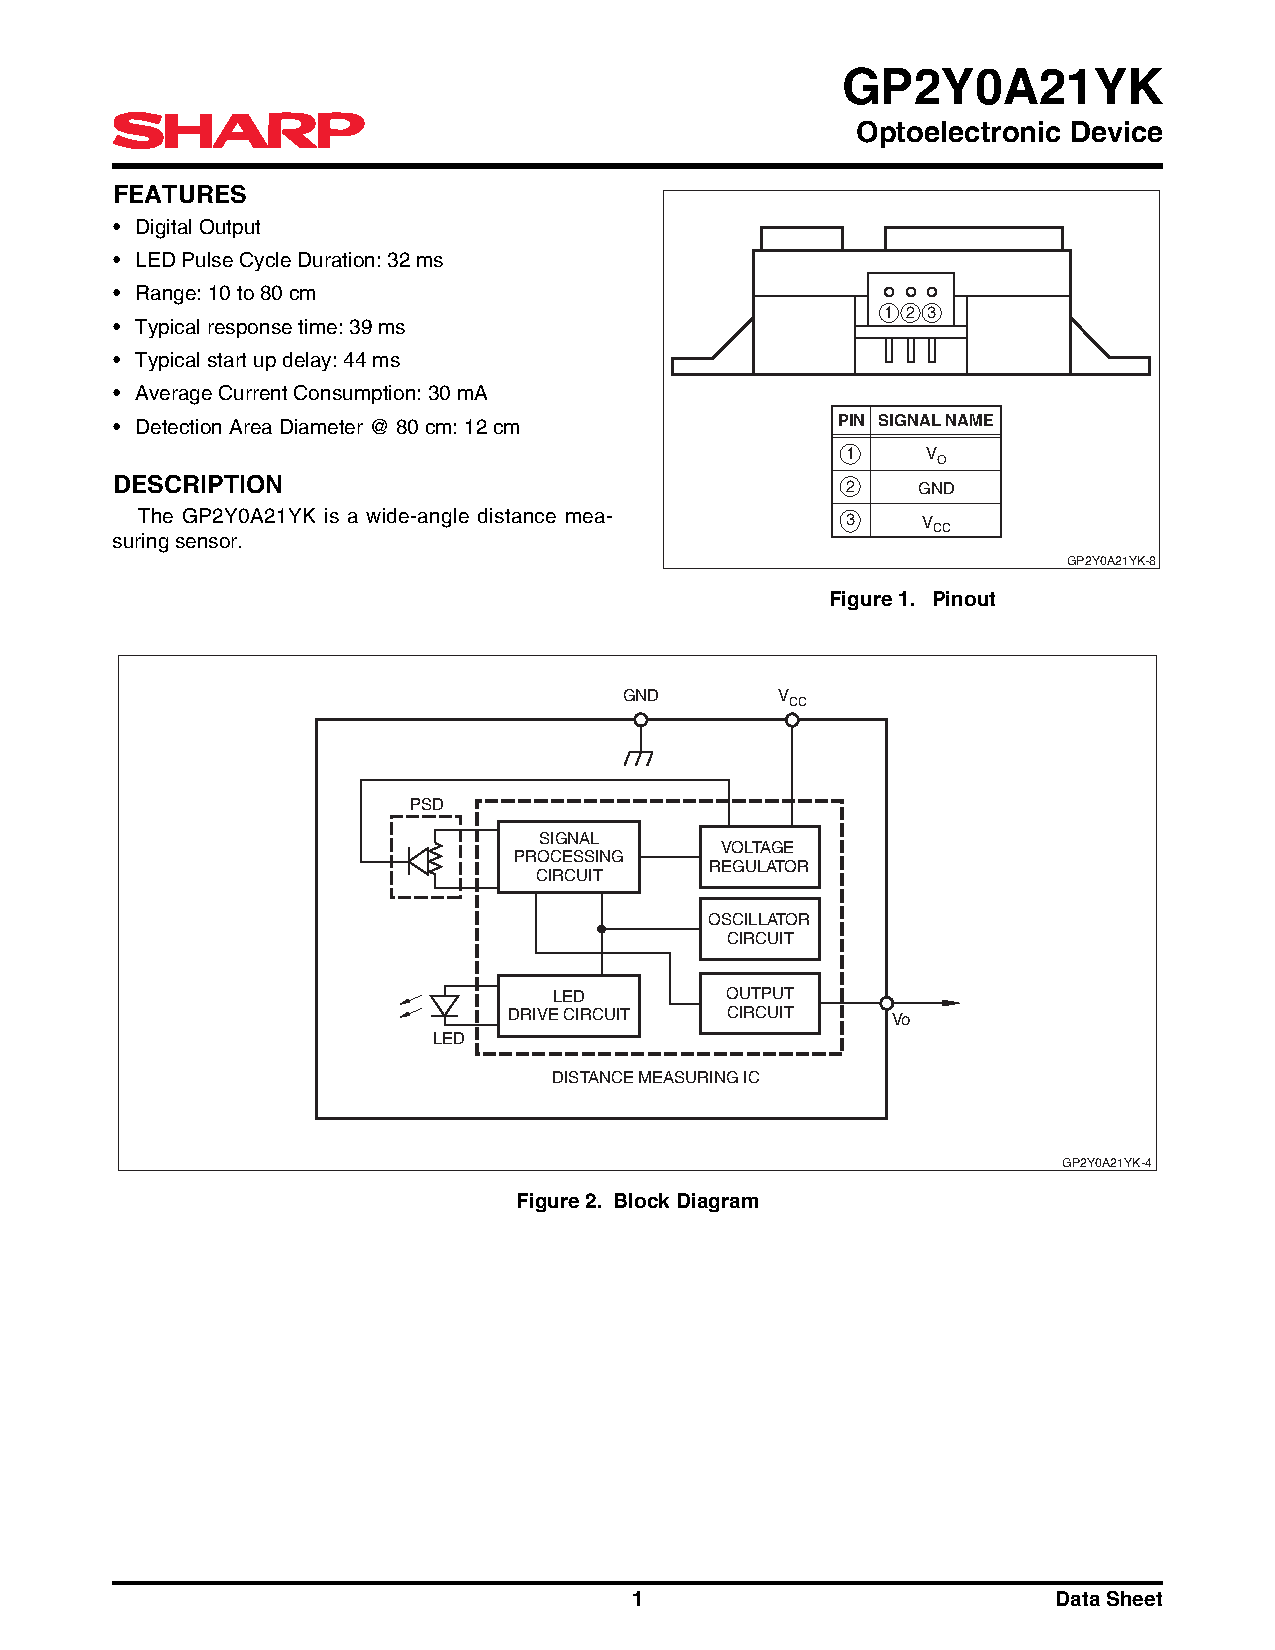
\includepdf[pages=1]{datasheets/SharpDatasheet.pdf}
%
%\cleardoublepage

%
%\chapter{Something Else}\label{sec:something}
%
%Add here some other appendix material \dots
%
% \cleardoublepage

\chapter{Messungen}

\begin{figure}[H]
\begin{tabular}{c|c||c|c|c|c|c|c|}
\cline{3-8}

\multicolumn{2}{c|}{} & \multicolumn{3}{c|}{$T = 650 ^\circ C$} & \multicolumn{3}{c|}{$T = 950 ^\circ C$} \\ \hline
\multicolumn{1}{|c|}{ $V_{in} $ }& $[nL/\text{min}]$ &1.0 & 1.5 & 2.0 & 1.0 & 1.5 & 2.0\\
\hline
\multicolumn{1}{|c|}{   $T_1$ }& $[^\circ C]$   & 366               & 363                 & 362               & 670.5             & 664                 & 660.5             \\ \hline
\multicolumn{1}{|c|}{        $T_2$ }& $[^\circ C]$   & 272.5             & 249.7               & 239.6             & 544.9             & 490                 & 463.8             \\ \hline
\multicolumn{1}{|c|}{        $T_3$ }& $[^\circ C]$   & 446.6                 & 439.6                   & 434.9                 & 762.4                 & 747.2                   & 738.9                 \\ \hline
\multicolumn{1}{|c|}{        $T_4$ }& $[^\circ C]$   & 451.9          & 444.2                   & 439.3                & 768.1                & 752                   & 744.1                 \\ \hline
\multicolumn{1}{|c|}{        $T_g$ }& $ [^\circ C]$   & 173.2             & 176.9               & 181.7             & 292.7             & 296.6               & 306.6             \\ 
\hline





\end{tabular}
\caption{Temperaturmessungen}
\label{tab:t1}
\end{figure}